% Licensed to the Apache Software Foundation (ASF) under one or more
% contributor license agreements. See the NOTICE file distributed with
% this work for additional information regarding copyright ownership.
% The ASF licenses this file to You under the Apache License, Version 2.0
% (the ``License''); you may not use this file except in compliance with
% the License. You may obtain a copy of the License at
%
% http://www.apache.org/licenses/LICENSE-2.0
%
% Unless required by applicable law or agreed to in writing, software
% distributed under the License is distributed on an ``AS IS'' BASIS,
% WITHOUT WARRANTIES OR CONDITIONS OF ANY KIND, either express or implied.
% See the License for the specific language governing permissions and
% limitations under the License.

\subsubsection{FileNet Job Options}

You must fill in four more tabs to configure a FileNet job.

\bigimage{fln-edit-job-tab3}

\ifJDBCGuide
% Licensed to the Apache Software Foundation (ASF) under one or more
% contributor license agreements. See the NOTICE file distributed with
% this work for additional information regarding copyright ownership.
% The ASF licenses this file to You under the Apache License, Version 2.0
% (the ``License''); you may not use this file except in compliance with
% the License. You may obtain a copy of the License at
%
% http://www.apache.org/licenses/LICENSE-2.0
%
% Unless required by applicable law or agreed to in writing, software
% distributed under the License is distributed on an ``AS IS'' BASIS,
% WITHOUT WARRANTIES OR CONDITIONS OF ANY KIND, either express or implied.
% See the License for the specific language governing permissions and
% limitations under the License.

\begin{itemize}
\label{scheduling}

\item \textbf{Schedule type:} Whether you want to scan every document
once or dynamically recrawl content in your repository. 

When scanning every document once, the crawler marks all documents that
have been previously crawled in this job as potentially to be deleted,
adds all seed documents to its queue and marks them as pending, processes
pending documents, marking them completed as they are ingested, and then
deleted all of the documents that were not recrawled. A document might
not be recrawled because it no longer exists, or the job specification
might have been changed to no longer include the document.

When dynamically recrawling documents, the crawler does not start by
marking all documents as potentially deletable; instead, it begins with
all of the seed documents, and continues adding to its list, periodically
re-adding the initial seed documents. If a document is removed from the
source, it will expire in the expiration interval (see below).

\item \textbf{Expiration Interval (if continuous):} The length of the
interval (in minutes) that the appliance will retain a document
crawled by this job after the document no longer appears in the
repository. After this interval, the missing document will be removed
from the appliance's index and archive. Leave the expiration interval
blank to keep missing documents indexed in GTS.

\item \textbf{Recrawl interval:} If you are dynamically recrawling
documents, how long, in minutes, the crawler should wait before
crawling documents a second time.

\item \textbf{Reseed interval:} If you are dynamically recrawling
documents, how long, in minutes, the crawler should wait before
looking for new documents to crawl. \ifMeridioGuide This connector
identifies all documents for ingestion through seeding; if the reseed
interval is infinite, the job will not ingest documents placed in the
repository during run time. (The job automatically reseeds whenever it
is started.) The default interval of 60 minutes is an appropriate
reseed rate. \fi \ifFilenetGuide This connector identifies documents
for ingestion during seeding. If you change the document inclusion
criteria, reseeding is required to identify new documents. Similarly,
documents placed in the repository while the job is running will not
be identified until the crawl is reseeded.  (The job automatically
reseeds whenever it is started.) The default interval of 60 minutes is
an appropriate reseed rate. \fi

\item \textbf{Scheduled time:} Allows you to define a time you wish
the job to run using a series of selection boxes. The first box refers
to the day of the week you wish the job to run, with an option to have
the job run any day of the week. The second box allows you to select
the start hour, with an option to start the job at any hour. The third
box allows you to specify which minute after the hour that you wish
the job to start. The fourth box allows you to specify what months of
the year you wish the job to run, with an option for the job to run
any month. The last box allows you to specify the day of the month you
wish the job to start, including any day of month.


You can scroll through each of the five boxes in this setting using
the arrow keys on your keyboard or by using the scroll bar on the
right side of the box.  If you want to select more than one value,
hold down control as you scroll and click the values that you want to
select. This allows you to define multiple windows with the same
length, for example by selecting Monday, Wednesday, and Friday at the
same time.

\item \textbf{Maximum run time:} The longest you will allow the job to
run, in minutes. For example, if you want to start a job at 2 AM but
force it to stop at 8 AM so that users have access to the repository,
you should set this value to 360 minutes. If the job is not complete by the
end time, documents that have already been found will be indexed, and
the rest of the crawl will continue at the beginning of the next
schedule interval. 

When you have defined the scheduled time and assigned a maximum run
time, click on the ``Add Scheduled Time'' button. A new schedule box
will appear below the scheduled time, allowing you to create
additional scheduled run times.

Here is a sample schedule for a job that will run every
Monday from 2 am to 6 am:

\begin{changemargin}{-.3in}{0in} 
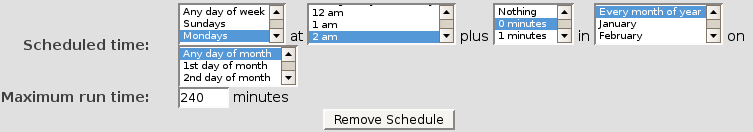
\includegraphics[width=300pt]{sample-schedule}
\end{changemargin}

If you do not have at least one scheduled time, the job will
only run when run manually (see page \pageref{ManageJobs}), and will
not automatically update the index on the appliance based on changes
to the repository.

You can remove a scheduled time by clicking the ``Remove Schedule''
button.

\end{itemize}

\fi

\ifCombinedConnectorGuide
This tab presents scheduling options. Here you can generate one or
more scheduled run times for the job. For a complete description of
the scheduling options, see the description starting on page
\pageref{scheduling}.
\fi

\bigimage{fln-edit-job-tab4}

Here on the Document Classes tab, you can configure which document
classes are ingested by this job, impose match conditions on documents
for ingestion based on metadata, and select which metadata will be
ingested with these documents. Each document class has its own section
on the tab with the following configuration options.

\begin{itemize}

\item \textbf{Include?}
Check this box to include this document class in your crawl.

\item \textbf{Document Criteria:}
Here you can place match conditions based on metadata that will limit
which documents are ingested. By default, all documents of the given
class are ingested if the ``Include'' box is checked.

Match expressions are created by selecting a metadata attribute, a
match type, and entering a match string. First, select any of the
metadata attributed to the document class to use in the match
expresssion from the selection box on the left. Using the drop down
box, select the desired match type. An ``Equals'' expression will
include all documents whose metadata attribute is equal to the match
string you specify in the text box on the right. A ``Not equals''
expression will include all documents whose metadata attribute is not
equal to the match string. A ``'Like' (with \% wildcards)'' expression
includes all documents whose metadata attribute is matched by a
wildcard match string. The \% wildcard matches zero or more
characters. You can use it to create match expressions such as
``\%Test\%'', which will match any string containing Test, or
``Test\%'', which will match any string beginning with Test.

Once you select a metadata attribute, a match type, and enter a match
string, click the ``Add'' button to the left of the expression. The
match expressions will appear above the selection area. You can
continue to add more match expressions. To delete a match expression,
simply click the delete box that appears to the left of each
expression.

\note{The ``Ingest?'' box must be selected for match expressions to apply.}

\item \textbf{Ingest all metadata fields?}
If you wish to ingest all metadata fields, simply check this box.

\item \textbf{Metadata fields:}
Use this box to select metadata fields for ingestion
individually. Hold the ``Shift'' key while clicking to select a
range. Hold the ``Ctrl'' key while clicking to allow multiple
selections. You can combine these effects.


\end{itemize}

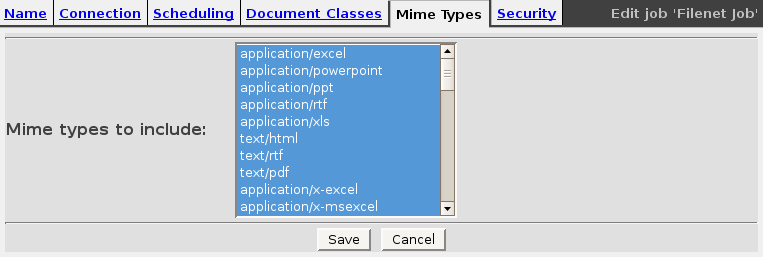
\includegraphics[width=300pt]{fln-edit-job-tab5}

\begin{itemize}

\item \textbf{Mime types to include:}
Here you can select which mime types to include in your searches from
a list of types generated by the appliance. Initially, all mime types
are selected. You can select a single type by clicking on it, which
clears all other selections. To keep previous selections, hold the
``Ctrl'' key while clicking. Holding the ``Shift'' key while clicking
allows you to select ranges. You can combine these effects to select
multiple ranges.


\end{itemize}

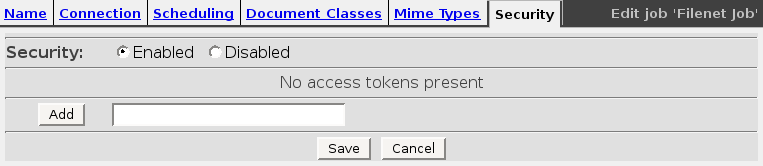
\includegraphics[width=300pt]{fln-edit-job-tab6}

\begin{itemize}



\item \textbf{Security:} Select ``Enabled'' to use Active Directory
permissions with the ingested documents. You can configure custom
permissions using the ``Access Tokens'' tools, or accept the ACLs
as given in the FileNet repository. Select ``Disabled'' to allow all
document search users to access to the files ingested by this job.

\note{If you wish to enforce security, your appliance should be joined
to an appropriate Active Directory domain.}

\item \textbf{Access Tokens:} This field allows you to create custom ACLs
for the files ingested by this job. Enter the SID of a user or group
that you wish to add to the custom ACLs for documents from this job,
then click the ``Add'' button. You can continue to add more SIDs. These
SIDs will appear in a list. Click the ``Delete'' button next to any SID
to remove it from the list.

\end{itemize}


After entering this information, you will be taken to the status page
for this job:

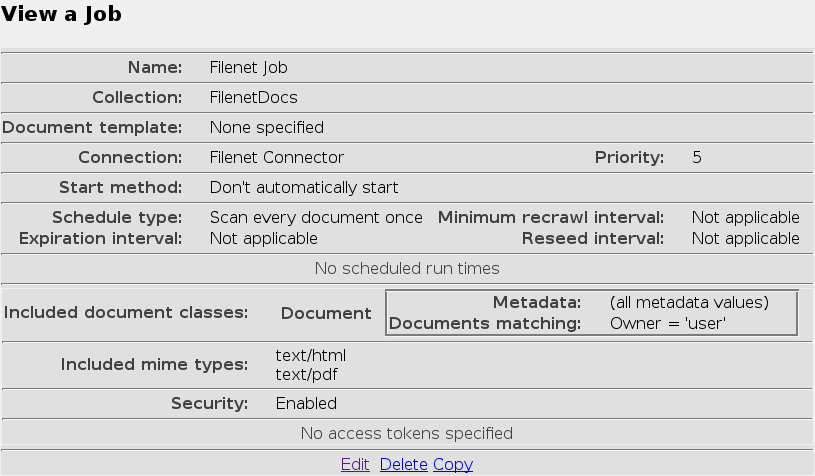
\includegraphics[width=300pt]{fln-view-job-status}


